\documentclass[../../D1.tex]{subfiles}

\begin{document}
\subsubsection{Neural Networks \& Deep Learning}
\emph{
    - Summary of NN\\
    - Structure of NN\\
    - Training \& Inference stages\\
    - weight update methodologies\\
    - Feed Forwards\\
    - Feedback Nerual Network\\
    - Self-organizing Neural Network\\
    - Weight parameters updated using back-propagation}


\begin{figure}
    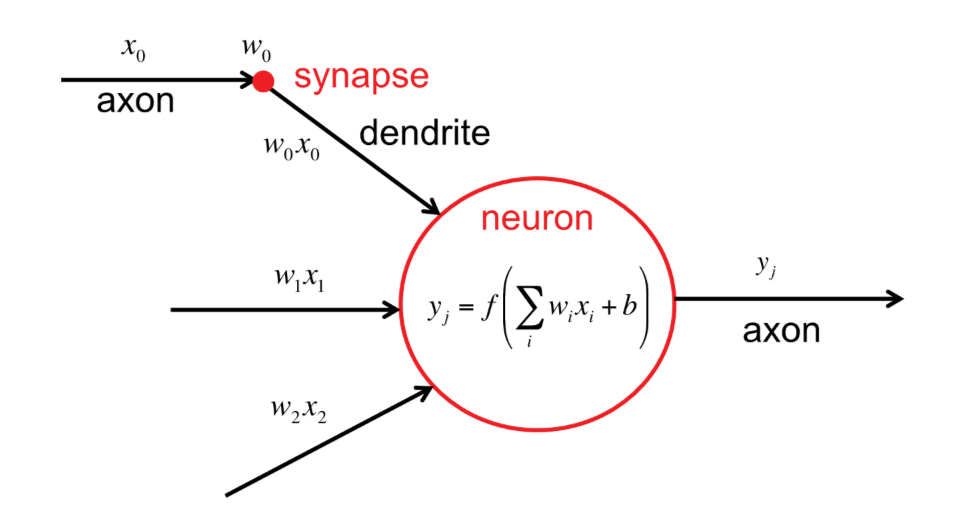
\includegraphics[width=1\textwidth]{Perceptron_efficient_proc.png}
    \caption{Neuron with corresponding biologically inspired labels.\\ \textbf{(Adopted figure from~\autocite{szeEfficientProcessingDeep2017})}}
    \label{fig:neuronLabeled}
\end{figure}
Deep learning is a subcategory of machine learning techniques where a hierarchy of layers perform some manner of information processsing with the goal of computing high level abstractions of the data by utilising low level abstractions identified in the early layers~\autocite{dengTutorialSurveyArchitectures2014}.


Neural networks fundamental purpose is to transform an input vector commonly referred to as~$X$ into an output vector~$\hat{Y}$. 
The output vector~$\hat{Y}$ is some form of classification such as a binary classification or a probability distribution over multiple classes~\autocite{thierry-miegHowFundamentalConcepts}. 
Between the input layer ($X$) and the output layer ($\hat{Y}$) there exists some number of interior layers that are referred to as hidden layers, the hidden and output layers are composed of neurons that pass signals derived from weights through the network, this model of computing was inspired by connectionism and our understanding of the human brain, see Fig.~\ref{fig:neuronLabeled} for labels of the analagous biological components. 
Weights in a neural network effectively correspond to the synapses in the brain and the output of the neruon is modelled as the axon. 
All neruons in a Neural network have weights corresponding to their inputs, these weights are are intended to mirror the value scaling effect of a synapse by performing a weighted sum operation~\autocite{szeEfficientProcessingDeep2017}.


Neural networks and deep neural networks are often reffered to interchangably, they are primarily distinguished by the number of layers, there is no hard rule indicating when a neural network is considered deep but generally a network with more than 3 hidden layers is considered a deep neural network, the rest of this dissertaion will refer to \acrshort{dnn}s for consistency. 
Each neuron in a \Acrshort{dnn} applies an non-linear activation function to the result of its weighted sum of inputs and weights, without which a \Acrshort{dnn} would just be a linear algebra operation~\autocite{szeEfficientProcessingDeep2017}, the cumulative effect of the activations in each layer results in elabourate causal chains of transormations than influence the aggregate activation of the network.

\textbf{Backpropagation} Although not the first to propose this approach~\autocite{schmidhuberDeepLearningNeural2015} the 1986 paper Learning representations by back-propagating errors~\autocite{rumelhartLearningRepresentationsBackpropagating1986} popularised back-propagation for updating weights during training multi-layer networks.

\Acrshort{dnn}s can be categorised as feedforwards, feedback, and self-organising networks depending on their processing method~\autocite{chenDeepLearningMobile2020}.


There are many popular deep neural network architectures, this document will continue to outline the \Acrshort{cnn} \& \Acrshort{rnn} architectures because these provide a high level overview of the type of models that will be used for the research posed in this dissertation.



\subsubsection{Convolutional Neural Networks}

\emph{Convolutional Neural Network (CNN)\\
    - A class of DNN\\
    - CNN consist of: Convolutional Layers, Pooling layers \& fully connected layers.\\
    - Convolutional Layers contain sets of filters/kernels}


Much like traditional nerual networks the \Acrshort{cnn} architecture was inspired by human and animal brains, the concept of processing the input with local receptive fields is conceptually similar some functionality of the cat's visual cortex~\autocite{hubelReceptiveFieldsBinocular1962,lecunConvolutionalNetworksImages,pouyanfarSurveyDeepLearning2019}. 
The influential paper by Hubel \& Weisel~\autocite{hubelReceptiveFieldsBinocular1962} ultimately had a significant influence on the design of \Acrshort{cnn}s via the Neocognitron, as proposed by Fukushima in~\autocite{fukushimaNeocognitronSelforganizingNeural1980} and again evaluated in~\autocite{fukushimaNeocognitronHierarchicalNeural1988}\textbf{(provide some comment on these papers)}. 

A critical aspect of image recognition is robustness to input shift and distortion, this robustness was indicated as one of the primary achivements of the Neocognitron in Fukushima's paper~\autocite{fukushimaNeocognitronSelforganizingNeural1980}. LeCunn and Bengio provide comprehensive explainations of how traditional \acrshort{dnn}s are so inefficient for these tasks 


The local receptive fields enable neurons to extract low level features such as edges, corners, and end-points with respect to their orientation. 
\Acrshort{cnn}s are robust to input shift or distortion by using receptive fields to identify these low level features across the entire input space, performing local averaging and downsampling in the layers following convolution layers means the absolute location of the features is less important than the position of the features relative to the position of other identified features~\autocite{lecunConvolutionalNetworksImages}. 
Each layer produces higher degrees of abstraction from the input layer, in doing so these abstractions retain important information about the input, these abstractions are referred to as feature maps.
The layers performing downsampling are known as pooling layers, they reduce the resolution or dimensions of the feature map which reduces overfitting and speeds up training by reducing the number of parameters in the network~\autocite{pouyanfarSurveyDeepLearning2019}.

Convolutional Networks for Images, Speech, and Time-Series by LeCunn \& Bengio


\acrshort{cnn}s have been found to be effective in many different AI domains, popular applications include: computer vision, \Acrshort{nlp}, and speech processing. 

\begin{figure}
    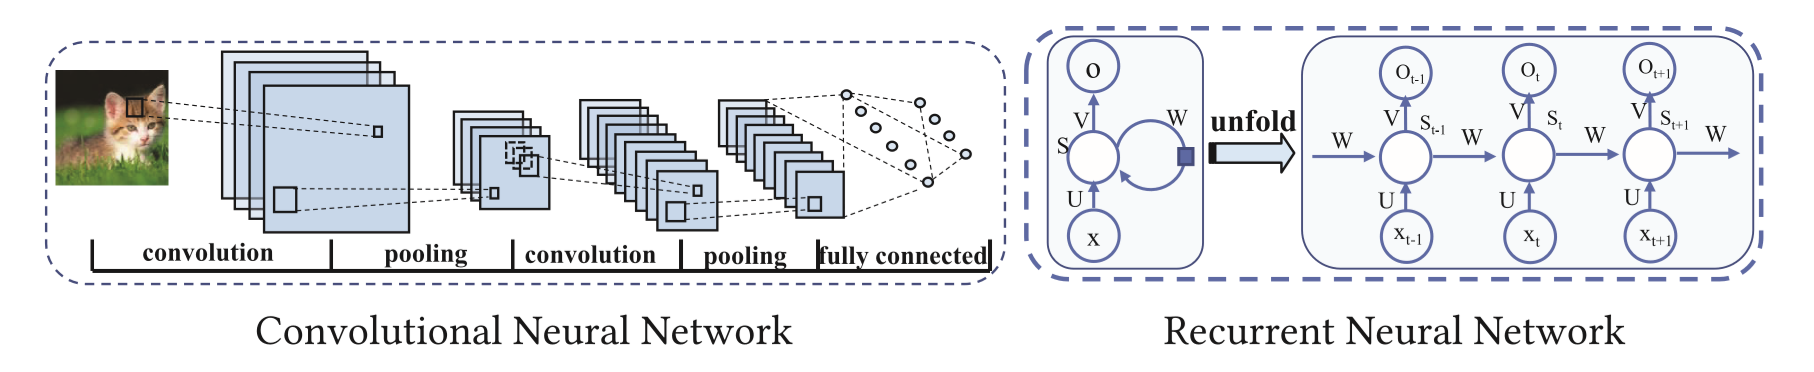
\includegraphics[width=1\textwidth]{CNN_RNN.png} 
    \caption{A typical example of a \acrshort*{cnn} (left) and \acrshort{rnn} (right)\\ \textbf{(Adopted figure from~\autocite{chenDeepLearningMobile2020})}}
    \label{fig:exampleCnnRnn}   
\end{figure}

\subsubsection{Recurrent Neural Netowrks}
\emph{Recurrent Neural Network (RNN)\\}
\acrshort{rnn}s are deep learning models that use loops in their layer connections to make predictions with sequential inputs and maintain state over those inputs, this architecture is designed specifically for time series predictions~\autocite{chenDeepLearningEdge2019}.


\end{document}